\section{Linear Programming}
\subsection{What's Linear Programming ?}
\begin{prettyBox}{Definition}{box} 
Linear programming is a sub-branch of optimization techniques. It involves modeling real-life problems as
linear equations and inequalities and using specialized methods to find optimal solution(s), if they exist.
\end{prettyBox}
\vspace{0.25cm}
\begin{center}
    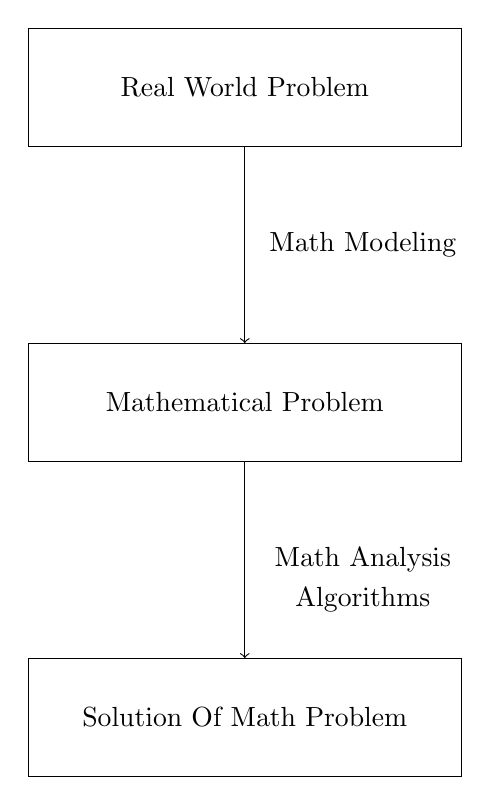
\begin{tikzpicture}
       \draw (0,0) rectangle (5.5,1.5);
       \node at (2.75,0.75) {Real World Problem};
      
       \draw[->] (2.75,0) -- (2.75,-2.5);
       \node at (4.25,-1.25) {Math Modeling};

       \draw (0,-4) rectangle (5.5,-2.5);
       \node at (2.75,-3.25) {Mathematical Problem};
      
       \draw[->] (2.75,-4) -- (2.75,-6.5);
       \node at (4.25,-5.25) {Math Analysis};
       \node at (4.25,-5.75) {Algorithms};
       
       \draw (0,-8) rectangle (5.5,-6.5);
       \node at (2.75,-7.25) {Solution Of Math Problem};
   \end{tikzpicture}
\end{center}
\vspace{1cm}
\subsection{Models}
\subsubsection{Graph Model}
This model is used when the objective function has two variables. It consists of converting all inequalities
into equalities, drawing them as lines, and then identifying the feasible area where all conditions are met.
We then sweep the objective function \(Z\) across the plot until we find the optimal solution(s).

\begin{prettyBox}{Note}{red}
 \textbf{\underline{Solutions : }}
When solving a linear program, the solution can be:
\begin{itemize}
    \item \textbf{One or Multiple Optimal Solutions}: The feasible area is a polygon, and its vertex points are the possible optimal solutions.
    \item \textbf{Infinitely Many Solutions}: If the solution is unbounded, then the objective function will increase or decrease infinitely as we sweep the line.
    \item \textbf{No Solution}: If the feasible area is empty (\{\(\emptyset\)\}), it indicates that the
system has contradictions.
\end{itemize}


\textbf{\underline{Direction of Increase/Decrease:}}

\begin{itemize}
    \item \textbf{Both Positive} \((a > 0\) , \(b > 0)\): Since both coefficients are positive, \( Z \) increases as
\( x_1 \) and \( x_2 \) increase, and decreases as they decrease. The direction of increase is towards the right,
and the direction of decrease is towards the left.

    \item \textbf{Both Negative} \((a < 0\) , \(b < 0)\): The opposite of the positive case. Here, \( Z \) increases
as \( x_1 \) and \( x_2 \) decrease, and decreases as they increase. The direction of increase is towards the left,
while the direction of decrease is towards the right.

    \item \textbf{Different Signs} \((a\) and \(b\) have opposite signs): The direction is determined by 
the coefficient with the larger absolute value, \(\max(|a|, |b|)\). If this coefficient is positive, the direction 
of increase follows the same pattern as when both coefficients are positive. If this coefficient is negative, 
the direction of increase follows the pattern for both negative coefficients.
\end{itemize}
\end{prettyBox}



\subsubsection*{{\underline{Example1 :} Diet Problem}}

\vspace{0.25cm}
The Goal is to minimize food cost but to meet the minimum daily nutrition requirement
\vspace{1cm}
\begin{center}
\begin{tabular}{|c|c|c|c|c|c|}
    \hline
    Food & Units & Protein & Vit c & Iron & Price\\
    \hline
    Apples & 1 med & 0.4 & 6 & 0.4 & 8\\
    \hline
    Banana & 1 med & 1.2 & 10 & 0.6 & 10\\
    \hline
\end{tabular}
\end{center}

\newpage

\begin{multicols}{2}
\textbf{\underline{Variables Definition:}}\\

Let \(x_1\) be the number of Daily Unit Appels.\\

Let \(x_2\) be the number of Daily Unit Banana.\\
\columnbreak

\textbf{\underline{Constraint:}} 

\[
\left\{
    \begin{array}{l}
        \forall x_1 , x_2 \geq 0 \quad \text{(Non-negative number of food item) ...C1}\\
        0.4x_1 + 1.2x_2  \geq 70 \quad \text{(Minimum Protein Daily) ...\textcolor{greenPlot}{C2}}\\ 
        6x_1 + 10x_2  \geq 50 \quad \text{(Minimum Vitamine c Daily) ...\textcolor{purplePlot}{C3}}\\
        0.4x_1 + 0.6x_2  \geq 12 \quad \text{(Minimum Iron Daily) ...\textcolor{orangePlot}{C4}}
   \end{array}
   \right.
\] 
\end{multicols}
\vspace{0.5cm}
\begin{prettyBox}{Objective Function}{box}
\[
f(x_i) = Z = 8x_1 + 10x_2  
\]
\begin{center}
The goal is to minimize food cost by minmizing \(f(x_i)\), while meeting the minimum daily nutrition .
\end{center}
\end{prettyBox}
\vspace{1cm} 
\textbf{\underline{Problem :}} Find the minimum of \(f(x_i)\) subject to the contraints\\

\vspace{1cm}
\begin{center}
\begin{tikzpicture}
    \begin{axis}[
        height = 9.5cm,
        width = 10cm,
        axis lines = middle,           % Ensures axes cross at (0, 0)
        xlabel=$x_1$, 
        ylabel=$x_2$, 
        xmin = -1, xmax = 200,           % Set x-axis range
        ymin = -1, ymax = 60,           % Set y-axis range
       ytick={0,10,...,70},             % Y-tick values
        xtick={0,50,...,200},
    ]
  \addplot [draw=none, fill=blueArea!25] coordinates {(175,0) (200,0) (200,60)(0,60)  (0,70/1.2) }; 
  \addplot[thick, mark=*,color = greenPlot] coordinates {(175,0) (0,70/1.2)};
  %\addplot[color=red]coordinates{(150,8.5) (141,5)};
  \addplot[thick, mark=*, color = purplePlot] coordinates {(50/6,0) (0,5)};
  \addplot[thick, mark=*, color = orangePlot] coordinates {(30,0) (0,20)};

  \addplot[thick,dashed,redPlot] coordinates {(0,100/10) (100/8,0)};
  \addplot[thick,dashed,redPlot] coordinates {(0,250/10) (250/8,0)};

  \addplot[thick,dashed,redPlot] coordinates {(0,400/10) (400/8,0)};

  \addplot[thick,dashed,redPlot] coordinates {(0,{700/1.2/10}) ({700/1.2/8},0)};
  \addplot[thick,dashed,redPlot] coordinates {(0,950/10) (950/8,0)};
  \addplot[thick,dashed,redPlot] coordinates {(0,1400/10) (1400/8,0)};
\end{axis}
\node at (7.5,-0.2){\small (175,0)};
\node at (-0.55,7.5){\small \((0,\frac{70}{1.2})\)};

\node at (1.35,1){\textcolor{orangePlot}{C4}};
\node at (-0.35,0.35){\textcolor{purplePlot}{C3}};
\node at (3.25,3.5){\textcolor{greenPlot}{C2}};
\node at (6.75,5.75){\textcolor{blueArea}{Feasible Area}};

\draw (11,1.5) rectangle (15.45,6);
\node at (11.5,5.5){\textcolor{orangePlot}{C4 :}};
\node at (13.65,5.5){\textcolor{orangePlot}{\(0.4x_1 + 0.6x_2  = 12 \)}};
\node at (11.5,4.75){\textcolor{purplePlot}{C3 :}};
\node at (13.5,4.75){\textcolor{purplePlot}{\(6x_1 + 10x_2 = 50\)}};
\node at (11.5,4){\textcolor{greenPlot}{C2 :}};
\node at (13.65,4){\textcolor{greenPlot}{\(0.4x_1 + 1.2x_2 = 70\)}};
\node at (11.35,3.25){\textcolor{redPlot}{Z}};
\node at (11.75,3.25){\textcolor{redPlot}{:}};
\node at (13.08,3.25){\textcolor{redPlot}{\(8x_1 + 10x_2\)}};

\draw[fill=blueArea!20] (11.2,2) rectangle (11.7,2.5);
\node at (13.25,2.25){\textcolor{blueArea}{Feasible Area}};

\end{tikzpicture}
\end{center}

\vspace{0.75cm} 
\begin{center}
    \begin{tabular}{|c|c|c|}
        \hline 
        Possible Solutions  & (0,\(\frac{70}{1.2})\) & (175,0)\\
        \hline 
        Objective Function & \(\frac{700}{1.2}\approx\) 583.33 & 1400\\
        \hline 
    \end{tabular}
\end{center}

\subsubsection*{\underline{Solution}}

The blue area in the plot represents the feasible region, so the optimal solution(s) must be within this area. Since
the objective function \( Z \) increases towards the right (due to both coefficients being positive) and we want to
minimize \( Z \), we need to sweep the objective function line towards the feasible area , and the first intresection 
between the objective function and one of the vertex points is the min the optimal solution . Therefore,the optimal 
solution is \((0, \frac{70}{1.2})\) with \( Z = 8 \times 0 + 10 \times \frac{70}{1.2} \approx 583.33 \).


\subsubsection*{\underline{Example2 :} Blending Model}

\vspace{0.25cm}
similar to the previous example , this time we have a farm that needs to feed their chicken , there are 2 feeds
, we need to minimize cost of the feeds while meeting the minimum nutrient requirement

\vspace{0.25cm}
\begin{center}
\begin{tabular}{|c|c|c|c|c|}
    \hline 
    Feed & Nut$_{A}$ & Nut$_{B}$ & Nut$_{C}$ & Cost\\
    \hline 
    1 & 3 & 7 & 3 & 10\\
    \hline 
    2 & 2 & 2 & 6 & 4\\
    \hline
    Min Require & 60 & 84 & 72 &\\
    \hline
\end{tabular}
\end{center}

\vspace{1cm}

\begin{multicols}{2}
\textbf{\underline{Variables Definition:}}\\

Let \(x_1\) be the number of Feed 1.\\

Let \(x_2\) be the number of Feed 2.\\
\columnbreak

\textbf{\underline{Constraint:}} 

\[
\left\{
    \begin{array}{l}
        \forall x_1 , x_2 \geq 0 \quad \text{(Non-negative number of feeds) ...C1}\\
        3x_1 + 2x_2  \geq 60 \quad \text{(Minimum Nut$_{A}$ Daily) ...\textcolor{greenPlot}{C2}}\\ 
        7x_1 + 2x_2  \geq 84 \quad \text{(Minimum Nut$_{B}$ Daily) ...\textcolor{purplePlot}{C3}}\\
        3x_1 + 6x_2  \geq 72 \quad \text{(Minimum Nut$_{C}$ Daily) ...\textcolor{orangePlot}{C4}}
   \end{array}
   \right.
\] 
\end{multicols}
\vspace{0.5cm}
\begin{prettyBox}{Objective Function}{box}
\[
f(x_i) = Z = 10x_1 + 4x_2  
\]
\begin{center}
The goal is to minimize feeds cost by minmizing \(f(x_i)\), while meeting the minimum daily nutrition .
\end{center}
\end{prettyBox}
\vspace{1cm} 
\textbf{\underline{Problem :}} Find the minimum of \(f(x_i)\) subject to the contraints\\
\vspace{0.75cm} 
\begin{center}
    \begin{tabular}{|c|c|c|c|c|}
        \hline 
        Possible Solutions  & (0,42) & (6,21) & (18,3) & (24,0)\\
        \hline 
        Objective Function & 168 & 144 & 192 & 240\\
        \hline 
    \end{tabular}
\end{center}


\vspace{1cm}
\begin{center}
\begin{tikzpicture}
    \begin{axis}[
        height = 9.5cm,
        width = 10cm,
        axis lines = middle,           % Ensures axes cross at (0, 0)
        xlabel=$x_1$, 
        ylabel=$x_2$, 
        xmin = -1, xmax = 30,           % Set x-axis range
        ymin = -1, ymax = 50,           % Set y-axis range
    %   ytick={0,10,...,70},             % Y-tick values
     %   xtick={0,50,...,200},
    ]
  \addplot [draw=none, fill=blueArea!25] coordinates {(0,50) (0,42) (6,21) (18,3) (24,0) (30,0) (30,50)}; 
  \addplot[thick, mark=*,color = greenPlot] coordinates {(0,30) (20,0)};
  %\addplot[color=red]coordinates{(150,8.5) (141,5)};
  \addplot[thick, mark=*, color = purplePlot] coordinates {(0,42) (12,0)};
  \addplot[thick, mark=*, color = orangePlot] coordinates {(24,0) (0,12)};

  \addplot[thick,dashed,redPlot] coordinates {(0,50/4) (5,0)};
  \addplot[thick,dashed,redPlot] coordinates {(0,90/4) (9,0)};
  \addplot[thick,dashed,redPlot] coordinates {(0,144/4) (14.4,0)};
  \addplot[thick,dashed,redPlot] coordinates {(0,168/4) (16.8,0)};

  \addplot[thick,dashed,redPlot] coordinates {(0,200/4) (20,0)};
  \addplot[thick,dashed,redPlot] coordinates {(0,240/4) (24,0)};
\end{axis}
%\node at (7.5,-0.2){\small (175,0)};
%\node at (-0.55,7.5){\small \((0,\frac{70}{1.2})\)};

\node at (-0.25,6.75){\small (0,42)};
\node at (6.45,-0.2){\small (24,0)};
\node at (1.5,3.25){\small (6,21)};
\node at (4.95,0.35){\small (18,3)};

\node at (1.45,1.25){\textcolor{orangePlot}{C4}};
\node at (3.65,-0.15){\textcolor{purplePlot}{C3}};
\node at (4,2){\textcolor{greenPlot}{C2}};
\node at (5.75,4.75){\textcolor{blueArea}{Feasible Area}};

\draw (11,1.5) rectangle (15.45,6);
\node at (11.5,5.5){\textcolor{orangePlot}{C4 :}};
\node at (13.5,5.5){\textcolor{orangePlot}{\(3x_1 + 6x_2  = 72 \)}};
\node at (11.5,4.75){\textcolor{purplePlot}{C3 :}};
\node at (13.5,4.75){\textcolor{purplePlot}{\(7x_1 + 2x_2 = 84\)}};
\node at (11.5,4){\textcolor{greenPlot}{C2 :}};
\node at (13.5,4){\textcolor{greenPlot}{\(3x_1 + 2x_2 = 60\)}};
\node at (11.35,3.25){\textcolor{redPlot}{Z}};
\node at (11.75,3.25){\textcolor{redPlot}{:}};
\node at (13.08,3.25){\textcolor{redPlot}{\(10x_1 + 4x_2\)}};

\draw[fill=blueArea!20] (11.2,2) rectangle (11.7,2.5);
\node at (13.25,2.25){\textcolor{blueArea}{Feasible Area}};

\end{tikzpicture}
\end{center}

\subsubsection*{\underline{Solution}}

The blue area in the plot represents the feasible region, so the optimal solution(s) must be within this area. Since
the objective function \( Z \) increases towards the right (due to both coefficients being positive) and we want to
minimize \( Z \), we need to sweep the objective function line towards the feasible area , and the first intresection 
between the objective function and one of the vertex points is the min the optimal solution . Therefore,the optimal 
solution is \((6, 21)\) with \( Z = 10 \times 6 + 4 \times 21 = 144 \).

\vspace{0.25cm}
\subsubsection*{\underline{If The Prices Changed}}
the price of feed1 is now 14 and feed2 remains the same 4 , the constraints don't change meaning the feasible region
also stays the same and the possible solutions (coordinates of the vertex points of the polygon) only thing that
changes is the objective function 

\vspace{0.5cm}
\begin{prettyBox}{New Objective Function}{box}
\[
f(x_i) = Z = 14x_1 + 4x_2  
\]
\begin{center}
The goal is to minimize feeds cost by minmizing \(f(x_i)\), while meeting the minimum daily nutrition .
\end{center}
\end{prettyBox}

\vspace{0.75cm} 
\begin{center}
    \begin{tabular}{|c|c|c|c|c|}
        \hline 
        Possible Solutions  & (0,42) & (6,21) & (18,3) & (24,0)\\
        \hline 
        Objective Function & 168 & 168 & 264 & 336\\
        \hline 
    \end{tabular}
\end{center}


\vspace{1cm}
\begin{center}
\begin{tikzpicture}
    \begin{axis}[
        height = 9.5cm,
        width = 10cm,
        axis lines = middle,           % Ensures axes cross at (0, 0)
        xlabel=$x_1$, 
        ylabel=$x_2$, 
        xmin = -1, xmax = 30,           % Set x-axis range
        ymin = -1, ymax = 50,           % Set y-axis range
    %   ytick={0,10,...,70},             % Y-tick values
     %   xtick={0,50,...,200},
    ]
  \addplot [draw=none, fill=blueArea!25] coordinates {(0,50) (0,42) (6,21) (18,3) (24,0) (30,0) (30,50)}; 
  \addplot[thick, mark=*,color = greenPlot] coordinates {(0,30) (20,0)};
  %\addplot[color=red]coordinates{(150,8.5) (141,5)};
  \addplot[thick, mark=*, color = purplePlot] coordinates {(0,42) (12,0)};
  \addplot[thick, mark=*, color = orangePlot] coordinates {(24,0) (0,12)};

  \addplot[thick,dashed,redPlot] coordinates {(0,50/4) (50/14,0)};
  \addplot[thick,dashed,redPlot] coordinates {(0,90/4) (90/14,0)};
  \addplot[thick,dashed,redPlot] coordinates {(0,144/4) (144/14,0)};
  \addplot[thick,dashed,redPlot] coordinates {(0,168/4) (168/14,0)};

  \addplot[thick,dashed,redPlot] coordinates {(0,200/4) (200/14,0)};
  \addplot[thick,dashed,redPlot] coordinates {(0,240/4) (240/14,0)};
\end{axis}
%\node at (7.5,-0.2){\small (175,0)};
%\node at (-0.55,7.5){\small \((0,\frac{70}{1.2})\)};

\node at (-0.25,6.75){\small (0,42)};
\node at (6.45,-0.2){\small (24,0)};
\node at (1.5,3.25){\small (6,21)};
\node at (4.95,0.35){\small (18,3)};

\node at (1.45,1.25){\textcolor{orangePlot}{C4}};
\node at (3.65,-0.15){\textcolor{purplePlot}{C3}};
\node at (4,2){\textcolor{greenPlot}{C2}};
\node at (5.75,4.75){\textcolor{blueArea}{Feasible Area}};

\draw (11,1.5) rectangle (15.45,6);
\node at (11.5,5.5){\textcolor{orangePlot}{C4 :}};
\node at (13.5,5.5){\textcolor{orangePlot}{\(3x_1 + 6x_2  = 72 \)}};
\node at (11.5,4.75){\textcolor{purplePlot}{C3 :}};
\node at (13.5,4.75){\textcolor{purplePlot}{\(7x_1 + 2x_2 = 84\)}};
\node at (11.5,4){\textcolor{greenPlot}{C2 :}};
\node at (13.5,4){\textcolor{greenPlot}{\(3x_1 + 2x_2 = 60\)}};
\node at (11.35,3.25){\textcolor{redPlot}{Z}};
\node at (11.75,3.25){\textcolor{redPlot}{:}};
\node at (13.08,3.25){\textcolor{redPlot}{\(10x_1 + 4x_2\)}};

\draw[fill=blueArea!20] (11.2,2) rectangle (11.7,2.5);
\node at (13.25,2.25){\textcolor{blueArea}{Feasible Area}};

\end{tikzpicture}
\end{center}

\vspace{1cm}


\subsubsection*{\underline{Observation}}
\begin{itemize}
    \item The value of the minimum or maximum of the objective function is unique, but there can be multiple coordinate solutions.
    \item The line through (0, 42) and (6, 21) represents a contour line, indicating that the value of \(Z\) is constant along this line.
    \item If \(P_1\) and \(P_2\) are both optimal solutions, they must be adjacent boundary corners of the feasible region.
    \item When there are multiple solutions, they form a segment of coordinates on the boundary (edge) of the feasible region, where each coordinate in that segment represents an optimal solution. In linear programming, we typically focus on the vertex points.
\end{itemize}

\vspace{0.5cm}
\begin{prettyBox}{Note}{red}
\textbf{\underline{Difference Between Multiple \& Infinite Solutions:}}

\vspace{0.25cm}
One might wonder about the difference between these two terms since even multiple solutions have an infinite
number of solutions. The difference is that in infinite solutions, the solution is unbounded, unlike multiple
solutions, which have their solutions on a finite segment. But as mentioned before, even though multiple solutions
have infinite solutions, we focus only on the boundary corner points (vertex points).
\end{prettyBox}

\newpage
\subsubsection*{\underline{Example :}} Minimize \(f(x,y) = x + y\)

\vspace{0.5cm}
Subject To :
\[
    \hspace{-13cm}
\left\{
    \begin{array}{l}
        x + y  \geq 10\\ 
        x + y  \leq 9\\
        x , y  \geq 0
    \end{array}
   \right.
\]

\subsubsection*{\underline{Solution :}}the system clearly contains a contradiction so there is no solution

\vspace{0.5cm}
\subsubsection*{\underline{Example :}} Maximize \(f(x,y) = x + y\)

\vspace{0.5cm}
Subject To :
\[
    \hspace{-13cm}
\left\{
    \begin{array}{l}
        2x + y  \geq 9\\ 
        x + 3y  \geq 10\\
        x , y  \geq 0
    \end{array}
   \right.
\]

\subsubsection*{\underline{Solution :}}As \(x,y \to +\infty\) , \(f\to +\infty\) , solution unbounded

\vspace{0.5cm}
\subsubsection*{\underline{Example :}}There is an industry that creates two types of boats, A and B. We want
to maximize the profit while adhering to the limitations of resources and labor.

\vspace{0.5cm}
\begin{center}
    \begin{tabular}{|c|c|c|c|c|}
        \hline
        Boat & \makecell{Aluminum \\ (lb)} & \makecell{Machine Time\\ (min)} & \makecell{Labor \\ (hr)} & \makecell{Profit \\ (\$)} \\
        \hline
        A & 50 & 6 & 3 & 50\\
        \hline
        B & 30 & 5 & 5 & 60\\
        \hline
        max & 2000 & 300 & 200 &\\
        \hline
    \end{tabular}
\end{center}
\newpage
\begin{multicols}{2}
\textbf{\underline{Variables Definition:}}\\

Let \(x_1\) be the number of boat A.\\

Let \(x_2\) be the number of boat B.\\
\columnbreak

\textbf{\underline{Constraint:}} 

\[
\left\{
    \begin{array}{l}
        \forall x_1 , x_2 \geq 0 \hspace{1.65cm} \text{(Non-negative number of boats) ...C1}\\
        50x_1 + 30x_2  \leq 2000 \quad \text{(Maximum Aluminium (lb)) ...\textcolor{greenPlot}{C2}}\\ 
        6x_1 + 5x_2  \leq 300 \hspace{0.85cm} \text{(Maximum Machine Time(min)) ...\textcolor{purplePlot}{C3}}\\
        3x_1 + 5x_2  \leq 200 \hspace{0.85cm} \text{(Maximum Labor(h)) ...\textcolor{orangePlot}{C4}}
   \end{array}
   \right.
\] 
\end{multicols}
\vspace{0.5cm}
\begin{prettyBox}{Objective Function}{box}
\[
f(x_i) = Z = 50x_1 + 60x_2  
\]
\begin{center}
The goal is to maximize the profits by maximizing \(f(x_i)\), while adhering to the ressource limitations .
\end{center}
\end{prettyBox}

\vspace{1cm}
\begin{center}
\begin{tikzpicture}
    \begin{axis}[
        height = 9.5cm,
        width = 10cm,
        axis lines = middle,           % Ensures axes cross at (0, 0)
        xlabel=$x_1$, 
        ylabel=$x_2$, 
        xmin = -1, xmax = 70,           % Set x-axis range
        ymin = -1, ymax = 70,           % Set y-axis range
    %   ytick={0,10,...,70},             % Y-tick values
     %   xtick={0,50,...,200},
    ]
  \addplot [draw=none, fill=blueArea!25] coordinates {(0,40) (25,25) (40,0) (0,0) }; 
  \addplot[thick, mark=*,color = greenPlot] coordinates {(0,200/3) (40,0)};
  %\addplot[color=red]coordinates{(150,8.5) (141,5)};
  \addplot[thick, mark=*, color = purplePlot] coordinates {(0,60) (50,0)};
  \addplot[thick, mark=*, color = orangePlot] coordinates {(200/3,0) (0,40)};

 \addplot[thick,dashed,redPlot] coordinates {(0,1000/60) (1000/50,0)};

 \addplot[thick,dashed,redPlot] coordinates {(0,500/60) (500/50,0)};

 \addplot[thick,dashed,redPlot] coordinates {(0,1600/60) (1600/50,0)};

 \addplot[thick,dashed,redPlot] coordinates {(0,2400/60) (2400/50,0)};

 \addplot[thick,dashed,redPlot] coordinates {(0,2000/60) (2000/50,0)};

 \addplot[thick,dashed,redPlot] coordinates {(0,2750/60) (2750/50,0)};

\end{axis}

\node at (0.75,4.75){\small (0,40)};
\node at (2.65,2.65){\small (25,25)};
\node at (5.25,0.35){\small (40,0)};

\node at (6.65,1.25){\textcolor{orangePlot}{C4}};
\node at (5.75,0.85){\textcolor{purplePlot}{C3}};
\node at (4,2){\textcolor{greenPlot}{C2}};
\node at (2.25,1.5){\textcolor{blueArea}{Feasible Area}};

\draw (11,1.5) rectangle (15.45,6);
\node at (11.5,5.5){\textcolor{orangePlot}{C4 :}};
\node at (13.5,5.5){\textcolor{orangePlot}{\(3x_1 + 5x_2  = 200 \)}};
\node at (11.5,4.75){\textcolor{purplePlot}{C3 :}};
\node at (13.5,4.75){\textcolor{purplePlot}{\(6x_1 + 5x_2 = 300 \)}};
\node at (11.5,4){\textcolor{greenPlot}{C2 :}};
\node at (13.75,4){\textcolor{greenPlot}{\(50x_1 + 30x_2 = 2000\)}};
\node at (11.35,3.25){\textcolor{redPlot}{Z}};
\node at (11.75,3.25){\textcolor{redPlot}{:}};
\node at (13.2,3.25){\textcolor{redPlot}{\(50x_1 + 60x_2\)}};

\draw[fill=blueArea!20] (11.2,2) rectangle (11.7,2.5);
\node at (13.25,2.25){\textcolor{blueArea}{Feasible Area}};

\end{tikzpicture}
\end{center}


\vspace{0.75cm} 
\begin{center}
    \begin{tabular}{|c|c|c|c|}
        \hline 
        Possible Solutions  & (0,40) & (25,25) & (40,0) \\
        \hline 
        Objective Function & 2400 & 2750 & 2000 \\
        \hline 
    \end{tabular}
\end{center}
\newpage
\subsubsection*{\underline{Solution}}

The blue area in the plot represents the feasible region, so the optimal solution(s) must be within this area. Since
the objective function \( Z \) increases towards the right (due to both coefficients being positive) and we want to
maximize \( Z \), we need to sweep the objective function line towards the right , and the last intresection 
between the objective function and one of the vertex points of the feasible region is the max the optimal solution . 
Therefore,the optimal solution is \((25, 25)\) with \( Z = 50 \times 25 + 60 \times 25 = 2750 \).

\vspace{0.5cm}
\subsubsection*{\underline{Example :}}An Industry produce two products , P1 and P2 ,they want to minimize the costs
of the ressources needed to create the product : raw material M$_{A}$(lb) \& M$_{B}$(lb) and the needed labour (hr)
while adhering the constraint set upon the ressources and minimum production 

\vspace{0.75cm} 
\begin{center}
    \begin{tabular}{|c|c|c|c|c|c|c|}
        \hline 
        Process  & Labour(hr) & M$_{A}$(lb) & M$_{B}$(lb)& & P1 & P2 \\
        \hline 
        1 & 20 & 160 & 30 & &35 & 55 \\
        \hline 
        2 & 30 & 100 & 35 & &45 & 42 \\
        \hline 
        3 & 10 & 200 & 60 & &70 & 0 \\
        \hline
        4 & 25 & 75 & 80 & &0 & 90\\
        \hline
        max & 1000 & 8000 & 4000 & min & 2100 & 1800\\
        \hline
        price & fixed salary & 3\$/lb & 7\$/lb & & & \\
        \hline
    \end{tabular}
\end{center}

\vspace{0.5cm}
\begin{multicols}{2}
\textbf{\underline{Variables Definition:}}\\

Let \(x_1\) be the process 1.

\vspace{0.15cm}
Let \(x_2\) be the process 2.

\vspace{0.15cm}

Let \(x_3\) be the process 3.

\vspace{0.15cm}
Let \(x_4\) be the process 4.

\columnbreak

\hspace{0.5cm}\textbf{\underline{Constraint:}} 

\[
\left\{
    \begin{array}{l}
        \forall x_1 , x_2 , x_3 , x_4 \geq 0 \hspace{1.65cm} \text{(Non-negative number of processes) ...\textcolor{redPlot}{C1}}\\
        20x_1 + 30x_2 + 10x_3 + 4x_4  \leq 1000 \quad \text{(Maximum Labor(hr)) ...\textcolor{greenPlot}{C2}}\\ 
        160x_1 + 100x_2 + 200x_3 + 75x_3   \leq 8000 \hspace{0.85cm} \text{(Maximum M$_{A}$(lb)) ...\textcolor{purplePlot}{C3}}\\
        30x_1 + 35x_2 + 60x_3 + 80x_4  \leq 4000 \hspace{0.85cm} \text{(Maximum M$_{B}$(lb)) ...\textcolor{blueArea}{C4}}\\
        35x_1 + 45x_2 + 70x_3 \geq 2100 \hspace{0.85cm} \text{(Minimum P1) ...\textcolor{pur}{C5}}\\
        55x_1 + 42x_2 + 90x_4  \geq 1800 \hspace{0.85cm} \text{(Minimum P2) ...\textcolor{orangePlot}{C6}}
   \end{array}
   \right.
\] 
\end{multicols}
\vspace{0.5cm}
\begin{prettyBox}{Objective Function}{box}
\[
f(x_i) = Z = 3\times(160x_1 + 100x_2 + 200x_3 + 75x_3) + 4\times(30x_1 + 35x_2 + 60x_3 + 80x_4)\\
           =690x_1 + 545x_2 + 1070x_3 + 785x_4
\]
\begin{center}
The goal is to minimize the cost by minimizing \(f(x_i)\), while adhering to the ressource limitations and
minimum production of P1 \& P2.
\end{center}
\end{prettyBox}

\vspace{0.5cm}
\subsubsection*{\underline{Example :}} Let's take the same problem as before but allow overtime max 200hr with
additional salary \$30/hr what's the new LP problem ? 

\vspace{0.5cm}
\begin{multicols}{2}
\textbf{\underline{Variables Definition:}}\\

Let \(x_1\) be the process 1.

\vspace{0.15cm}
Let \(x_2\) be the process 2.

\vspace{0.15cm}
Let \(x_3\) be the process 3.

\vspace{0.15cm}
Let \(x_4\) be the process 4.

\vspace{0.15cm}
Let \(y\) be the number of overtime hour

\columnbreak

\hspace{0.5cm}\textbf{\underline{Constraint:}} 

\[
\left\{
    \begin{array}{l}
        \forall x_1 , x_2 , x_3 , x_4 \geq 0 \hspace{1.65cm} \text{(Non-negative number of processes) ...\textcolor{redPlot}{C1}}\\
        20x_1 + 30x_2 + 10x_3 + 4x_4  \leq 1000 + y \quad \text{(Maximum Labor(hr)) ...\textcolor{greenPlot}{C2}}\\ 
        y \leq 200 \quad \text{(Maximum Overtime(hr)) ...\textcolor{yellow}{C3}}\\
        y \geq 0 \quad \text{(Overtime cant be negative) ...\textcolor{brown}{C4}}\\
        160x_1 + 100x_2 + 200x_3 + 75x_3   \leq 8000 \hspace{0.85cm} \text{(Maximum M$_{A}$(lb)) ...\textcolor{purplePlot}{C5}}\\
        30x_1 + 35x_2 + 60x_3 + 80x_4  \leq 4000 \hspace{0.85cm} \text{(Maximum M$_{B}$(lb)) ...\textcolor{pur}{C6}}\\
        35x_1 + 45x_2 + 70x_3 \geq 2100 \hspace{0.85cm} \text{(Minimum P1) ...\textcolor{blueArea}{C7}}\\
        55x_1 + 42x_2 + 90x_4  \geq 1800 \hspace{0.85cm} \text{(Minimum P2) ...\textcolor{orangePlot}{C8}}
   \end{array}
   \right.
\] 
\end{multicols}
\vspace{0.5cm}
\begin{prettyBox}{Objective Function}{box}
\[
g(x_i) = Z = f(x_i) + 30y =  690x_1 + 545x_2 + 1070x_3 + 785x_4 + 30y
\]
\begin{center}
The goal is to minimize the cost by minimizing \(g(x_i)\), while adhering to the ressource limitations and
minimum production of P1 \& P2.
\end{center}
\end{prettyBox}

\vspace{0.5cm}
\subsubsection*{\underline{Example :}}The transportation model setting , good at location A$_{i}$, transport 
to B$_{j}$ cost from A$_{i}$ Tp B$_{j}$, the goal is to find a schedule to minimize the cost 
At location A$_{1}$ we have 200 units , location A$_{2}$ we have 300 units , the will be distriuted to 
B$_{1}$ ,B$_{2}$, B$_{3}$ :

B$_{1}$ = 100units ,B$_{2}$ = 200units , B$_{3}$ = 200units

\vspace{0.2cm}
Transportation cost from A$_{i}$ to B$_{j}$ :

\begin{center}
    \begin{tabular}{|c|c|c|c|}
        \hline
        & B$_{1}$ & B$_{2}$ & B$_{3}$\\
        \hline 
        A$_{1}$ & 11 & 12 & 13 \\
        \hline 
        A$_{2}$ & 21 & 22 & 23\\
        \hline
    \end{tabular}
\end{center}

\newpage
\begin{multicols}{2}
\textbf{\underline{Variables Definition:}}\\[2.5cm]
Let \(x_{ij}\) be the number of transported Units from A$_{i}$ to B$_{j}$.

\columnbreak

\hspace{0.5cm}\textbf{\underline{Constraint:}} 

\[
\left\{
    \begin{array}{l}
        \forall x_{ij} \geq 0 \hspace{1.65cm} \text{(Non-negative number of units) ...\textcolor{redPlot}{C1}}\\
    i = \{1,2\} \quad,\quad j = \{1,2,3\}\\
         x_{11} + x_{12} + x_{13}  = 200 \quad \text{(Maximum Capacity of A$_{1}$) ...\textcolor{greenPlot}{C2}}\\ 
         x_{21} + x_{22} + x_{23}  = 300 \quad \text{(Maximum Capacity of A$_{2}$)...\textcolor{purplePlot}{C3}}\\
         x_{11} + x_{21} = 100 \quad \text{(Maximum Capacity of B$_{1}$)...\textcolor{orangePlot}{C4}}\\
         x_{12} + x_{22} = 200 \quad \text{(Maximum Capacity of B$_{2}$)...\textcolor{blueArea}{C5}}\\
         x_{13} + x_{23} = 200 \quad \text{(Maximum Capacity of B$_{3}$)...\textcolor{pur}{C6}}
   \end{array}
   \right.
\] 
\end{multicols}
\vspace{0.5cm}
\begin{prettyBox}{Objective Function}{box}
\[
    f(x_i) + 30y =  11x_{11} + 12x_{12} +13x_{13} +21x_{21} +22x_{22} +23x_{23} 
\]
\begin{center}
The goal is to minimize the cost of transport by minimizing \(f(x_i)\), while adhering to the capacity limitation
\end{center}
\end{prettyBox}

\vspace{0.5cm}

\begin{prettyBox}{Note}{red}
Constraint can be  : \(= , \leq , \geq ,> ,<\)

We can rewrite any constraint into a  \textbf{Standard Form}
\end{prettyBox}

\subsection{Standard Form} 
The standard form is a structured way of representing LP problems. It helps
to standardize diverse problems, making them easier to analyze and solve using
models like the Simplex Method and primal-dual relationships. Converting
problems to standard form ensures uniformity, simplifying both theoretical 
understanding and computational implementation.

\begin{prettyBox}{}{box}
\[
    \text{Maximize } Z = c_1x_1 + c_2x_2 + \cdots + c_nx_n
\]

\vspace{0.25cm}
\hspace{1cm}\text{Subject to:}
\[
\begin{aligned}
    a_{11}x_1 + a_{12}x_2 + \cdots + a_{1n}x_n &= b_1 \\
    a_{21}x_1 + a_{22}x_2 + \cdots + a_{2n}x_n &= b_2 \\
    &\hspace{-2cm}\vdots \\
    a_{m1}x_1 + a_{m2}x_2 + \cdots + a_{mn}x_n &= b_m
\end{aligned}
\]

\[
    x_1, x_2, \dots, x_n \geq 0 \hspace{0.35cm} b_1, b_2, \dots, b_m \geq 0 
\]
\end{prettyBox}

\subsubsection{How To Transition To Standard Form}


\begin{prettyBox}{Minimization Problem}{box}
In the standard form, all linear programming problems must be expressed as maximization problems. If we are given a minimization problem, 
we can convert it by multiplying the objective function by \(-1\), effectively turning it into a maximization problem.
\end{prettyBox}

\subsubsection*{\underline{Example}}
\[
\text{Minimize } f(x_i) = 3x_1 + 2x_2
\]
is equivalent to:
\[
\text{Maximize } g(x_i) = -f(x_i) = -3x_1 - 2x_2
\]

\vspace{0.5cm}
\begin{prettyBox}{Constraints}{box}
In the standard form , all constraints are equalities , if a contraint is not an equality
we have to add or substract new positive variables called slack variables\\[0.25cm]
\boldsymbol{\leq} \textbf{Constraint}
\begin{equation*}
x \leq b \Leftrightarrow x + s_1 = b \quad \text{with} \quad s_1 \geq 0
\end{equation*}
\boldsymbol{\geq} \textbf{Constraint}
\begin{equation*}
    x\geq b \Leftrightarrow x-s_1=b \quad \text{with} \quad s_1\geq 0
\end{equation*}
\end{prettyBox}

\subsubsection*{\underline{Example}}

\[
\left\{
\begin{array}{l}
    x_{1} + x_{2} + x_{3} \leq 100 \\
    x_{1} - x_{2} \geq 5 \\
    x_{1}, x_{2}, x_{3} \geq 0
\end{array}
\right.
\quad
\Longrightarrow
\quad
\left\{
\begin{array}{l}
    x_{1} + x_{2} + x_{3} + s_{1} = 100 \\
    x_{1} - x_{2} - s_{2} = 5 \\
    x_{1}, x_{2}, x_{3}, s_{1}, s_{2} \geq 0
\end{array}
\right.
\]


\vspace{1cm}
\subsection{Simplex Method}
The Simplex method, an algebraic iterative algorithm developed by B. Dantzig
in 1948, allows us to solve linear programming (LP) problems even those involving more 
than two variables. The principle of the method is to start from an initial feasible 
solution and iteratively move along the vertices of the polyhedron (feasible area) until the optimal solution
is reached.

\subsection*{\underline{Overview Of Simplexe Steps}}

\vspace{0.35cm}
\begin{center}
    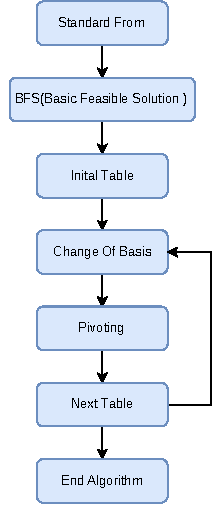
\includegraphics[height=0.9\textheight]{Chapters/Diagram/simplexe.drawio.pdf}
\end{center}


\subsubsection{BFS}

\begin{prettyBox}{Basic Feasible Solution}{box}
After converting the \textbf{LP} problem into standard form, the next step is to find a basic feasible solution. 
To achieve this, set all decision variables to 0 and assign the slack variables the values of the right-hand side (\textbf{RHS}) of the constraints.\\[0.15cm]
If any slack variable equals \(-\text{\textbf{RHS}}\), an artificial variable must be added to satisfy the non-negativity constraint for slack variables. 
In this case, the slack variable is set to 0, and the artificial variable is assigned the RHS value.\\[0.2cm]
For example: 
\[
x_1 + x_2 - s_1 = 10 \quad \Longrightarrow \quad x_1 + x_2 - s_1 + t_1 = 10
\]

where \(t_1 \geq 0\) is the artificial variable added to the equation.
\end{prettyBox}

\vspace{0.25cm}

\begin{prettyBox}{Coefficient Of Objective Function}{red}
The coefficient of artificial variables in the objective function is \(-M\),
where \(M\) is a very large number, ensuring that artificial variables are
driven out of the basis during the optimization process.\\[0.15cm]
The coefficient of slack variables is 0.
\end{prettyBox}

\vspace{0.25cm}
\begin{prettyBox}{Basic/Non-Basic}{red}
In the context of the Basic Feasible Solution (BFS), the variables that 
are non-zero are referred to as \textbf{basic variables}, while the remaining
variables are called \textbf{non-basic variables}.
\end{prettyBox}


\vspace{1cm}

\subsubsection{Initial Table}
\begin{prettyBox}{Create Initial Table}{box}
\[
    \text{Maximize } Z = c_1x_1 + c_2x_2 + \cdots + c_nx_n
\]

\vspace{0.25cm}
\hspace{1cm}\text{Subject to:}
\[
\begin{aligned}
    a_{11}x_1 + a_{12}x_2 + \cdots + a_{1n}x_n &= b_1 \\
    a_{21}x_1 + a_{22}x_2 + \cdots + a_{2n}x_n &= b_2 \\
    &\hspace{-2cm}\vdots \\
    a_{m1}x_1 + a_{m2}x_2 + \cdots + a_{mn}x_n &= b_m
\end{aligned}
\]

\[
    x_1, x_2, \dots, x_n \geq 0 \quad b_1, b_2, \dots, b_m \geq 0 
\]
\end{prettyBox}

\newpage
The notation for vectors and matrices is as follows:

\[
X = \left[\begin{matrix} x_1 & x_2 & \dots & x_n \end{matrix}\right], \hspace{0.35cm}
C = \left[\begin{matrix} c_1 & c_2 & \dots & c_n \end{matrix}\right], \hspace{0.35cm}
b = \left[\begin{matrix} b_1 \\ b_2 \\ \vdots \\ b_m \end{matrix}\right], \hspace{0.35cm}
B = \left[\begin{matrix} B_1 \\ B_2 \\ \vdots \\ B_m \end{matrix}\right], \hspace{0.35cm}
C_B = \left[\begin{matrix} cb_1 \\ cb_2 \\ \vdots \\ cb_m \end{matrix}\right]
\]

\vspace{0.5cm}

\[
A = \left[\begin{matrix} a_{11} & \dots & a_{1n}\\
                           \vdots & & \vdots\\
                           a_{m1} & \dots & a_{mn}\end{matrix}\right]
\]


\vspace{0.75cm}
\[
Z_1 = C_B \cdot b \quad \text{and} \quad Z_i = C_B \cdot A(:, i-1) \quad \text{for} \quad i \geq 2 
\]

\vspace{0.5cm}
Where:
\begin{itemize}
    \item \( n \) is the number of variables.
    \item \( m \) is the number of constraints.
    \item \( b \) is the vector of right-hand side (RHS) values.
    \item \( X \) is the vector of variables.
    \item \( C \) is the vector of coefficients in the objective function.
    \item \( A \) is the matrix of coefficients in the constraints.
    \item \( A(:,i-1) \) is submatrix of A all rows of column\(_{i-1}\)
    \item \( B \) is the vector of basic variables.
    \item \( C_B \) is the vector of the coefficients of the objective function for the basic variables.
    \item \( Z_1 \) is the value of the objective function.
\end{itemize}

\vspace{0.5cm}

\begin{prettyBox}{Reminder: Dot Product}{red}
    \[U = \left[\begin{matrix} u_1 & u_2 & \dots & u_m \end{matrix}\right] ,
\hspace{0.3cm}
    V = \left[\begin{matrix} v_1 & v_2 & \dots & v_m \end{matrix}\right]\]

\vspace{0.15cm}
\[U \cdot V = u_1.v_1 + u_2.v_2 + \dots + u_m.v_m\]
\end{prettyBox}

\begin{center}
    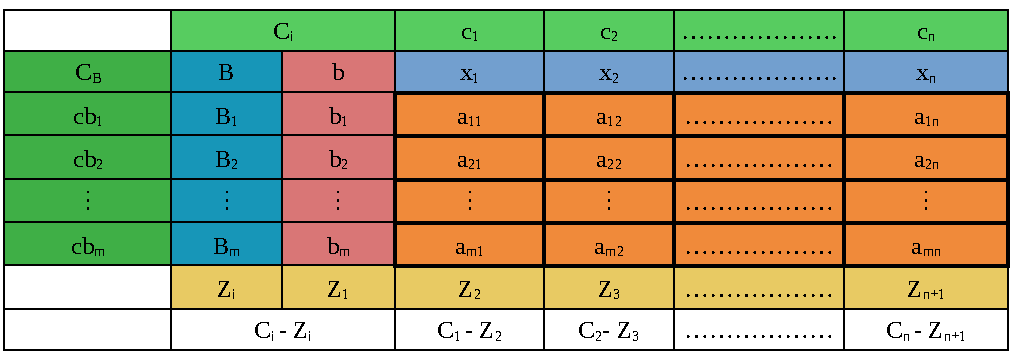
\includegraphics{Chapters/Simplexe/table.pdf}
\end{center}

\vspace{0.25cm}

\begin{center}
    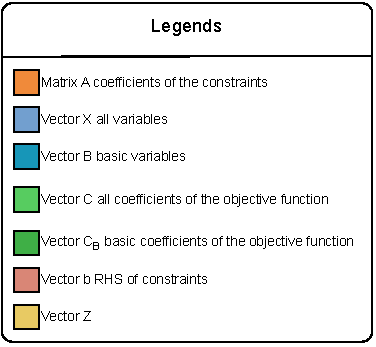
\includegraphics[width=0.45\textwidth]{Chapters/Simplexe/leg.drawio.pdf}
\end{center}

\subsubsection{Change of Basis}
\begin{prettyBox}{Changing the Basis}{box}
To change the basis, follow these steps:
\begin{enumerate}
    \item Choose a non-basic variable to enter the basis.
    \item Choose a basic variable to leave the basis.
\end{enumerate}
\end{prettyBox}


\begin{prettyBox}{Choose Variable to Enter the Basis}{box}
    Select the column where \(C_i - Z_{i+1} > 0\) and is at its maximum. This column is called the 
\textbf{pivoting column}, and \(x_i\) is the variable that will enter the basis.
\end{prettyBox}

\vspace{0.35cm}

\begin{prettyBox}{Choose Variable to Leave the Basis}{box}
Select the line where \(a_{ji} > 0\) and \(\frac{b_j}{a_{ji}}\) is at its minimum (where \(i\) is the pivoting column). This line is called the \textbf{pivoting line}, and 
\(B_i\) is the basic variable that will leave the basis.
\end{prettyBox}
\vspace{0.35cm}
\begin{prettyBox}{Note}{red}
    The intersection of the pivoting column and the pivoting line is called the \textbf{pivot} which is \(a_{ji}\).
\end{prettyBox}

\vspace{0.35cm}
\begin{center}
    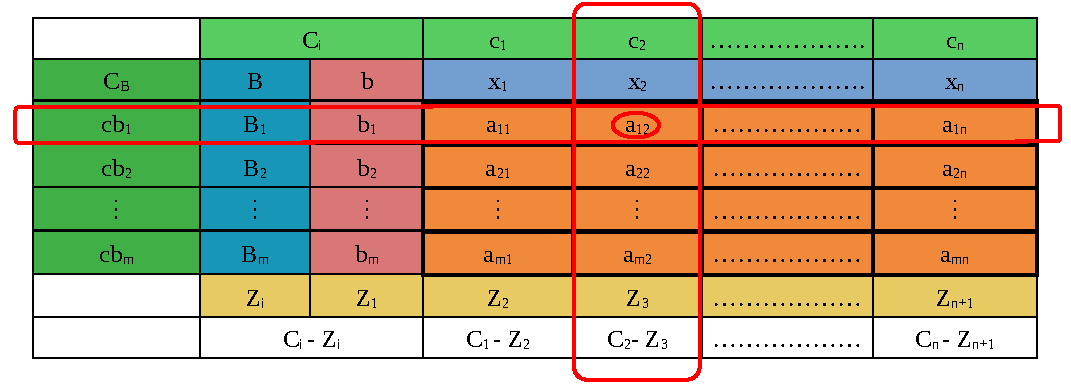
\includegraphics{Chapters/Simplexe/basis.pdf}
\end{center}

\begin{itemize}   
    \item In this case the max of\hspace{0.2cm}\(C_i - Z_{i+1} > 0\)\hspace{0.2cm}is\hspace{0.2cm}\(C_2 - Z_3\)\hspace{0.35cm} i = 2 so \(x_2\) 
will be the variable to enter the basis.
\item The min of \hspace{0.1cm}\(\frac{b_j}{a_{ji}}\)\hspace{0.1cm} with \(a_{ji} > 0\)\hspace{0.1cm} is \hspace{0.1cm} \(\frac{b_1}{a_{12}}\)\hspace{0.35cm} j = 1 so \(B_1\)
will leave the basis
\item The intersection between the pivoting line and pivoting column is \(a_{12}\)
 
\end{itemize}



\subsubsection{Pivoting}
\begin{prettyBox}{Pivoting}{box}
To get the new table, follow these steps:
\begin{enumerate}
    \item Replace \(B_j\) with \(x_i\).
    \item Divide all the elements of the pivoting line by the pivot value (excluding \(C_B\) and \(B\)).
    \item Set all cells above or below the pivot to 0.
    \item Fill the remaining cells using the rectangle rule:
        \[
        a = a' - \frac{b \times c}{\text{pivot}}
        \]
        where:
        \begin{itemize}
            \item \(a\): New value of the cell.
            \item \(a'\): Old value of the cell.
            \item \(b\): Intersection of the cell's row with the pivoting column.
            \item \(c\): Intersection of the cell's column with the pivoting row.
        \end{itemize}
\end{enumerate}
\end{prettyBox}

\vspace{0.5cm}

\begin{prettyBox}{Note}{red}
\begin{itemize}
    \item If a cell in the pivoting column is 0 (\(b = 0\)), the entire row intersecting with it stays the same.
    \item If a cell in the pivoting line is 0 (\(c = 0\)), the entire column intersecting with it stays the same.
\end{itemize}
\end{prettyBox}

